\PassOptionsToPackage{unicode}{hyperref}
\PassOptionsToPackage{hyphens}{url}
\documentclass{article}
\setcounter{secnumdepth}{6}

\usepackage{amsmath,amssymb}
\usepackage{lmodern}
\usepackage{iftex}
\usepackage[letterpaper, margin=1in, top=0.5in, bottom=1in]{geometry}
\usepackage{listings}
\usepackage{color}
\usepackage{titling}
\usepackage{graphicx}
\usepackage{hyperref}

\ifPDFTeX
  \usepackage[T1]{fontenc}
  \usepackage[utf8]{inputenc}
  \usepackage{textcomp} 
\else 
  \usepackage{unicode-math}
  \defaultfontfeatures{Scale=MatchLowercase}
  \defaultfontfeatures[\rmfamily]{Ligatures=TeX,Scale=1}
\fi
\IfFileExists{upquote.sty}{\usepackage{upquote}}{}
\IfFileExists{microtype.sty}{
  \usepackage[]{microtype}
  \UseMicrotypeSet[protrusion]{basicmath} 
}{}
\makeatletter
\@ifundefined{KOMAClassName}{
  \IfFileExists{parskip.sty}{
    \usepackage{parskip}
  }{
    \setlength{\parindent}{0pt}
    \setlength{\parskip}{6pt plus 2pt 2pt}}
}{
  \KOMAoptions{parskip=half}}
\makeatother
\usepackage{xcolor}
\usepackage{graphicx}

\makeatletter
\def\maxwidth{\ifdim\Gin@nat@width>\linewidth\linewidth\else\Gin@nat@width\fi}
\def\maxheight{\ifdim\Gin@nat@height>\textheight\textheight\else\Gin@nat@height\fi}
\makeatother
\setkeys{Gin}{width=\maxwidth,height=\maxheight,keepaspectratio}
\makeatletter
\def\fps@figure{htbp}
\makeatother
\setlength{\emergencystretch}{3em} 
\providecommand{\tightlist}{
  \setlength{\itemsep}{0pt}\setlength{\parskip}{0pt}}

\ifLuaTeX
  \usepackage{selnolig}  
\fi
\IfFileExists{bookmark.sty}{\usepackage{bookmark}}{\usepackage{hyperref}}
\IfFileExists{xurl.sty}{\usepackage{xurl}}{} 
\urlstyle{same}
\hypersetup{
  hidelinks,
  pdfcreator={LaTeX via pandoc}}

\title{Artifacts - Sprint 5}
\date{}

\begin{document}

\maketitle

\hypertarget{sos-s3} {
\section{Scrum of Scrums}\label{Scrum of Scrums} 
At this point, the team was organized to move forward on the console and the Pacman Game.
We mainly updated the UML diagram of the PACMAN game in terms of coalitions, scoring, sprites, movement process and we managed to implement the Game Communication in the Client and Server sockets. Then, in the Daily Lead's we made a conclusion on the pacman UML diagram to move forward on the dependent tasks also on the bridge.jar implementations and finally we finished with a conclusion on what we expect from SOCKETS to use in the library. 
}

\href{https://github.com/Pending-Name-21/arquitecture/pull/11}{Link: UML-Pacman Game - Pull Request on GitHub}.

\href{https://github.com/Pending-Name-21/arquitecture/pull/17}{Link: Game-Comunication - Pull Request on GitHub}.

\begin{figure}
\centering
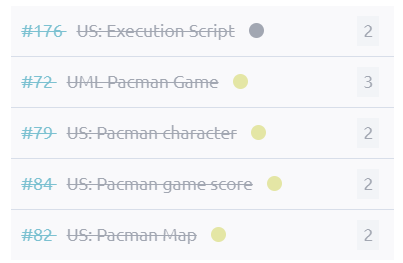
\includegraphics[width=16cm, height=10cm]{./assets/US-Sprint5.png}
\end{figure}

\hypertarget{burndownchart-s3}{
\section{Burn Down Chart}\label{Burn Down Chart S3}}
\href{https://tree.taiga.io/project/joseluis-teran-coffeetime/taskboard/sprint-5-3817}{Link: Sprint 5 Board on Taiga}.

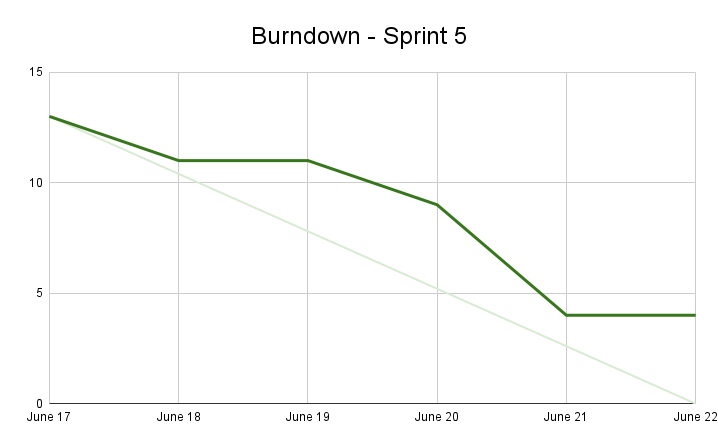
\includegraphics[width=\textwidth]{./assets/Burndown-Sprint5.png}

\hypertarget{startstopcontinueactionitems-s3}{
\section{Start-Stop-Continue-Action Items}\label{Start-Stop-Continue-Action Items S6}}
\href{https://miro.com/app/board/uXjVKDO7l8M=/?moveToWidget=3458764590247999187&cot=14}{Link: Start-Stop-Continue-Action Items Sprint 5 on Miro}.

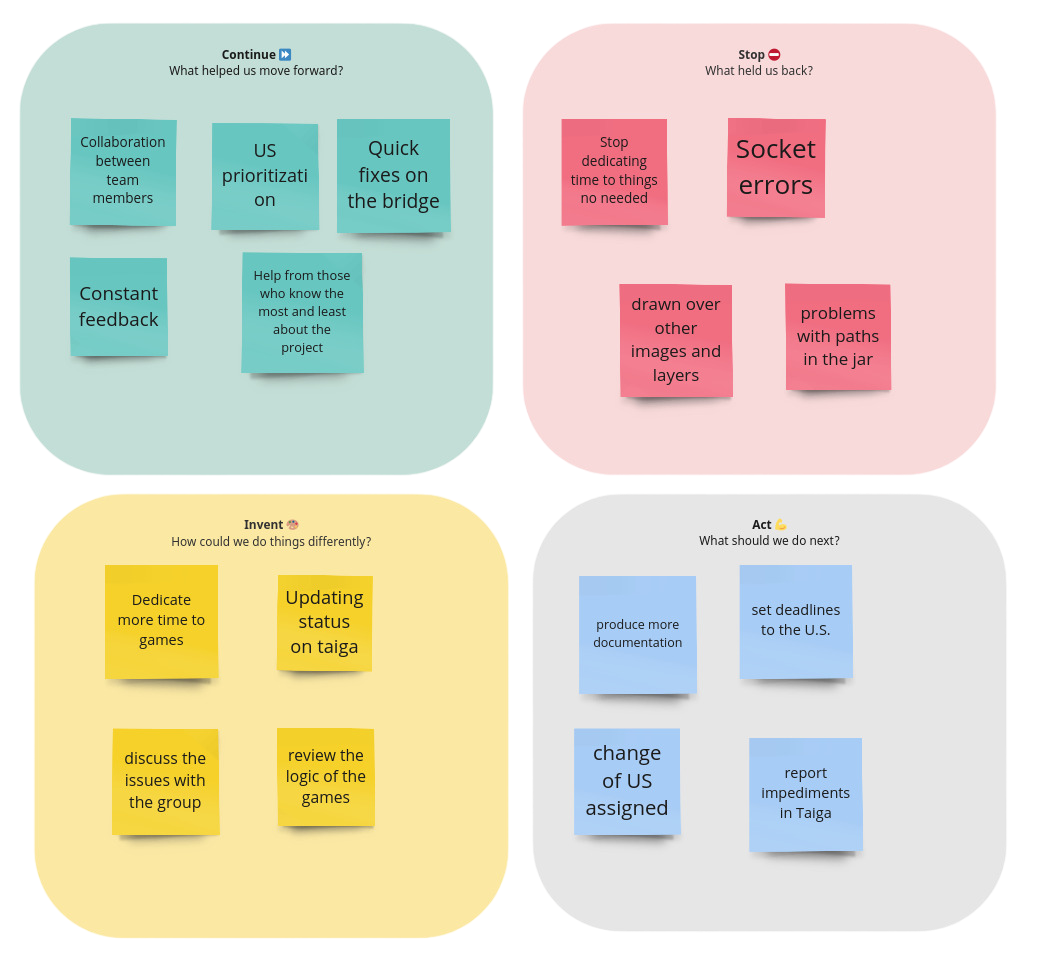
\includegraphics[width=\textwidth]{./assets/Retrospectives-Sprint5.png}

\end{document}
